%!TEX encoding = UTF-8 Unicode
% options:
% thesis=B bachelor's thesis
% thesis=M master's thesis
% czech thesis in Czech language
% slovak thesis in Slovak language
% english thesis in English language
% hidelinks remove colour boxes around hyperlinks

\documentclass[thesis=M,czech]{FITthesis}[2012/06/26]

\usepackage[utf8]{inputenc} % LaTeX source encoded as UTF-8

\usepackage{graphicx} %graphics files inclusion
\graphicspath{ {img/} }
% \usepackage{amsmath} %advanced maths
% \usepackage{amssymb} %additional math symbols


\usepackage{caption}
\usepackage{subcaption}


\usepackage{dirtree} %directory tree visualisation

% % list of acronyms
% \usepackage[acronym,nonumberlist,toc,numberedsection=autolabel]{glossaries}
% \iflanguage{czech}{\renewcommand*{\acronymname}{Seznam pou{\v z}it{\' y}ch zkratek}}{}
% \makeglossaries

\newcommand{\tg}{\mathop{\mathrm{tg}}} %cesky tangens
\newcommand{\cotg}{\mathop{\mathrm{cotg}}} %cesky cotangens

% % % % % % % % % % % % % % % % % % % % % % % % % % % % % % 
% ODTUD DAL VSE ZMENTE
% % % % % % % % % % % % % % % % % % % % % % % % % % % % % % 

\department{Katedra \ldots (DOPLŇTE)}
\title{Doplňte název práce Žluťoučký á kůň aaa}
\authorGN{Doplňte Vaše křestní jméno/jména} %(křestní) jméno (jména) autora
\authorFN{Doplňte Vaše příjmení} %příjmení autora
\authorWithDegrees{Doplňte Vaše jméno a tituly} %jméno autora včetně současných akademických titulů
\supervisor{Doplňte jméno vedoucího práce}
\acknowledgements{Doplňte, máte-li komu a za co děkovat. V~opačném případě úplně odstraňte tento příkaz.}
\abstractCS{V~několika větách shrňte obsah a přínos této práce v~češtině. Po přečtení abstraktu by se čtenář měl mít čtenář dost informací pro rozhodnutí, zda chce Vaši práci číst.}
\abstractEN{Sem doplňte ekvivalent abstraktu Vaší práce v~angličtině.}
\placeForDeclarationOfAuthenticity{V~Praze}
\declarationOfAuthenticityOption{4} %volba Prohlášení (číslo 1-6)
\keywordsCS{Nahraďte seznamem klíčových slov v češtině oddělených čárkou.}
\keywordsEN{Nahraďte seznamem klíčových slov v angličtině oddělených čárkou.}

\begin{document}

% \newacronym{CVUT}{{\v C}VUT}{{\v C}esk{\' e} vysok{\' e} u{\v c}en{\' i} technick{\' e} v Praze}
% \newacronym{FIT}{FIT}{Fakulta informa{\v c}n{\' i}ch technologi{\' i}}

\begin{introduction}
	%sem napište úvod Vaší práce
\end{introduction}

\chapter{Cíl práce}
\cite{svgspec}

% POUŽITÉ METODY -------------------------------------------------------------------------------------------------------------------------------------------------------------------------------------------------------------
\chapter{Použité metody}
\section{Dobývání znalostí z databází (KDD)}
\textit{Dobývání znalostí z databází (Knowledge discovery in databases, KDD)} představuje netriviální extrakci nových a reálně využitelných znalostí z dat\cite{kddb}. 

Cílem KDD je získat cenné nové informace, které nebyly z neopracovaných dat explicitně viditelné a vhodným způsobem a formou pak tyto informace zobrazit, popřípadě využít v reálných systémech.\cite{fayyad}

KDD se dá popsat jako proces skládající se z několika kroků. Tyto kroky se zpravidla iterativně opakují a některé vyžadují vysokou interakci uživatele. Kroky KDD, tak jak jsou popsány v \cite{hbcap}, jsou následující:

\begin{figure}[htbp]
\begin{center}
	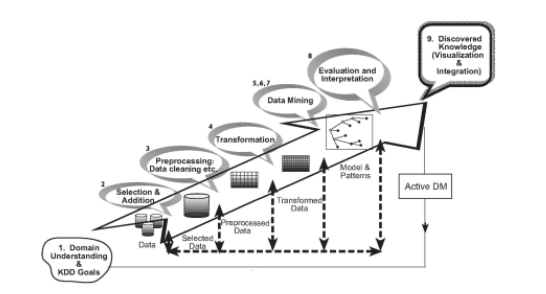
\includegraphics[scale=0.75]{kdd_steps}
\caption{Kroky KDD podle \cite{fayyad}}
\end{center}
 \captionsetup{font={footnotesize,bf,it}}
  \caption*{zdroj: \cite{fayyad}}
\end{figure}

\subsubsection*{Porozumění aplikační doméně a stanovení cílů}
Částí počátečního kroku je důkladně poznat aplikační doménu. Další kritickou částí je stanovení cílů, které by KDD měly přinést koncovému uživateli. Tato rozhodnutí pak významným způsobem ovlivňují jednotlivá rozhodnutí v dalších krocích.
 		
\subsubsection*{Výběr dat}
Potom, co je specifikován cíl, je zapotřebí rozhodnout z jakých dat se budou znalosti dobývat. 
Výsledkem tohoto kroku je vstupní množina dat, která velmi ovlivňuje úspěch celého KDD. Pokud například budou chybět některé významné atributy, s ohledem na stanovený cíl, celý proces pravděpodobně nebude úspěšný. Z tohoto pohledu je dobré zahrnout co nejvíce různých atributů. Na druhou stranu s velikostí dat se zvyšuje výpočetní a prostorová náročnost napříč metodami ze všech následujících kroků. Tyto protichůdné požadavky je třeba zvážit a udělat kompromis. Správnému rozhodnutí by měla pomoci iterativní povaha celého procesu.

\subsubsection*{Předzpracování}
Tento krok má za cíl zvýšit kvalitu dat. Předzpracování by se mělo například vypořádat s chybějícími a odlehlými hodnotami. Nejen v tomto kroku platí \uv{\emph{garbage in garbage out}}, koncept běžný pro počítačové vědy a matematiku, který stojí na myšlence, že kvalita výstupu je určena kvalitou vstupu\cite{g_in_g_out}.

\subsubsection*{Transformace }
\label{subsec:transformace}

V této části KDD se používají metody na transformaci atributů, jako je například diskretizace. Dále se v tomto kroku může měnit dimenzionalita dat a to buď zmenšovat metodami jako \textit{feature selection, feature extraction}, nebo naopak zvětšovat odvozovováním atributů nových. 


\subsubsection*{Datamining}
Před tímto krokem bychom měli mít k dispozici připravená data. Jak již bylo ovšem zmíněno, celý process KDD je iterativní a tento krok lze provádět s různými datovými sadami a výsedky vzájemně porovnávat.

Ze stanoveného cíle KDD jsou odvozeny kritéria pro zvolení vhodných dataminingových metod. Zvolené metody se poté aplikují na připravená data. Výsledkem tohoto kroku může být natrénovaný model nebo sada extrahovaných znalostí.

\subsubsection*{Vyhodnocení a interpretace}
V této časti máme již natrénované modely, popřípadě extrahované znalosti. Tyto výsledky musíme vyhodnotit a interpretovat z hlediska cílů, které byly stanoveny v prvním kroku.

\subsubsection*{Využití}
Využití je posledním krokem celého KDD. Získané znalosti jsou využity v reálných systémech a natrénované modely jsou nasazeny do produčního prostředí. Tento krok se snaží přinést užitek koncovému uživateli. Úspěch tohoto kroku definuje úspěch celého KDD.	
	

\subsection{Datamining}
Jak bylo zmíněno v předchozí kapitole, datamining je jedna z částí dobývání znalostí z databází. V první části této kapitoly jsou popsány některé třídy úloh podle \cite{fayyad}, které jsou metody dataminingu schopné řešit. V druhé části jsou představeny základní metody spolu s nastíněním jejich využitelnosti k řešení jednotlivých typů úloh. 

\begin{description}
    \item[Klasifikace]
    
    je druh problému určení kategorie, do které dané pozorování patří. Proces dataminingu tak spočívá v učení funkce, která zobrazuje datové vektory do jedné z předdefinovaných tříd. Klasifikaci je možné uplatnit naříklad na následující problém: pracovník 
    banky má rozhodnout zda poskytnout žadateli půjčku. O žadateli má banka spoustu informací, stejně tak jako o dalších klientech, kteří si již v minulosti u banky peníze půjčili a poté je vrátili (nebo nevrátili).
    
    
    \item[Regrese]
    
    je podobná třída úloh jako klasifikace s rozdílem, že na výstupu se neobjevuje kategorie pozorování, nýbrž reálná proměnná. Jde tak o učení funkce, která mapuje datové vektory do reálné proměnné. Předpovídání atributů (jako např.: teplota, věk, cena, velikost \dots) na základě historických dat je typický příklad pro regresi.
    

   \item[Shlukování]
   
   je úloha, při které je snaha hledat a identifikovat konečný počet shluků, kterým lze popsat data. Jedná se tak o opačný přístup, než u klasifikace, kde máme třídy dat dopředu známé. Shluková analýza může například odpovědět na otázku, jáké typy zákazníků kupují jaké produkty.
   
\end{description}


 \section{Metody dataminingu}
Všechny popisované metody předpokládají, že vstupní objeky jsou popsány sadou atributů a míra podpobnosti těchto atributů určuje míru příslušnosti k nějakému konceptu (například třídě). Takto popsaný objekt můžeme chápat jako bod v n-dimenzionálním prostoru. Výstupem metod jsou pak modely, které mapují tento prostor a reprezentují tak hledané znalosti.
Zmíněné metody se pak liší v následujícíh vlastnostech:


\begin{itemize}
\item vhodnost pro uvažovaný typ úlohy,
\item do jaké míry jsou nalezené znalosti srozumitelné pro uživatele,
\item síla metody -- jak jsou nalezené znalosti efektivní při klasifikaci nových případů, popřípadě jak složité shluky dokáží výsledky reprezentovat,
\item pro jaký typ dat jsou vhodné.
\end{itemize}

%Další společná vlastnost metod je, že využívají technik strojového učení. Strojové učení je podoblast umělé inteligence, která se zabývá algoritmy, které umožňují počítačovému systému “učit se”. V tomto kontextu je učení myšleno schopnost adaptovat vnitřní stav systému na vnější podněty bez explicitního naprogramování.

Jedna z možností, jak dělit metody je podle způsobu učení. První způsob je \textit{učení s učitelem}. V tomto způsobu učení je k dispozici dvojice vstupu a výstupu. Model se snaží aproximovat takto nadefinovanou funkci. Naproti tomu \textit{učení bez učitele} informace o požadovaném výstupu nemá. V následujících odstavcích budou popsáni vybraní představitelé těchto metod.\cite{eurokomise}

 \subsection{Metody učení s učitelem}
 \subsubsection*{Naive Bayes}
 \subsubsection*{KNN}
  \subsubsection*{Trees}
   
   
  \subsubsection*{MLP}
    \textit{Multilayer perceptron (MLP)} je druh dopředné umělé neuronové sítě.
Stavební prvky takové sítě jsou inspirovány biologickými neurony, tedy základní funkční jednotkou nervové tkáně. Umělé neurony reagují na vstupní signály a podle vnitřních vlastností signál šíří dál. Takové umělé neurony plně pospojované do orientovaného grafu pak tvoří MLP, která je využitelná v úlohách klasifikace a regrese. 

Tento orientovaný graf je organizován do vrstev -- zpravidla vstupní, jedna skrytá a výstupní vrstva (obr. \ref{fig:mlp}). V dopředných sítích, jako je MLP, se signál šíří striktně jedním směrem od vstupu, přes skryté vrstvy až po výstup. 

Pro konkrétní nastavení vah a jeden vstup síť reprezentuje analyticky vyjádřitelnou funkci. Protože se MLP učí s učitelem, máme k dispozici požadovaný výstup. Pokud definujeme funkci E jako vzdálenost mezi požadovaným a spočteným výstupem pro současné nastavení vah v síti, můžeme pomocí gradientu funkce E podle vah zjistit, jak upravit váhy pro zmenšení chyby. To se pak několikrát opakuje pro všechna dostupná vstupní data. 

MLP se uplatňují při řešení problémů jako je rozpoznávání obrazu a řeči a další. Jednou z nevýhod takových sítí je obtížná interpretace pro koncového uživatele, obvzláště v případech, kdy jsou sítě MLP využity jako podpora lidského rozhodování \cite{needed}. 

% vzorec backpropagation
% dopřednost
% Výhody (aproximace libovolné funkce)


\begin{figure}[htbp]
\begin{center}
	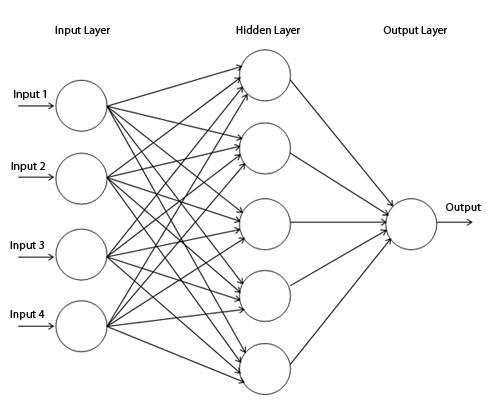
\includegraphics[scale=0.6]{mlp.jpeg}
\caption{Architektura MLP s jednou skrytou vrstvou}
\label{fig:mlp}
\end{center}
 \captionsetup{font={footnotesize,bf,it}}
  \caption*{zdroj: https://github.com/cazala/synaptic/wiki/Architect}
\end{figure}

 
 \subsection{Metody učení bez učitele}
  \subsubsection*{Hierarchical clustering}
  \subsubsection*{K-means}
 
\section{SOM}
Self organizing map (SOM), samoorganizující mapa, je umělá neuronová síť navržena Teuvo Kohonenem v 80. letech minulého století. Narozdíl od MLP se SOM skládá z jedné vrstvy speciálně uspořádaných neuronů. Dalším rozdílem je, že se učí bez učitele a to pomocí tzv. \textit{kompetitivní učení}.\cite{junkie}

\subsection{Struktura sítě}
SOM se typicky skládá z jedné vrstvy neuronů uspořádaných do pravidelné 2D nebo 3D mřížky. Topologie takové mřížky bývá zpravidla pravidelná a to hexagonání nebo pravoúhlá (obr. \ref{fig:top}). Složky vstupu jsou propojeny se všemi neurony.
Stejně jako dopředné sítě, SOM má ve spojích uložené váhy. Tuto skutečnost je však názornější zachycovat jako tzv.: \textit{prototypové vektory}, které jsou uloženy u jednotlivých neuronů. Každý prototypové vektor  má stejnou dimenzi jako je dimenze vstupních dat.

\begin{figure}
\centering
\begin{subfigure}{.5\textwidth}
  \centering
  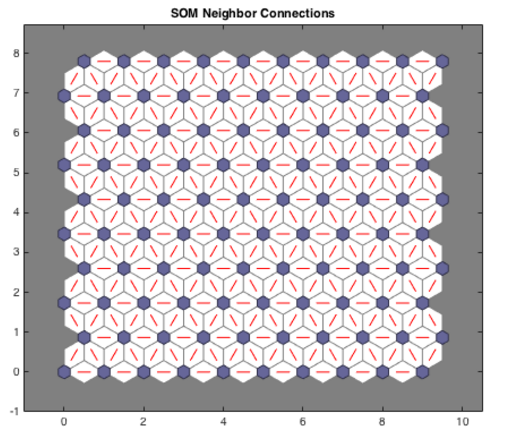
\includegraphics[width=.8\linewidth]{hex_top}
  \caption{Hexagonální topologie}
  \label{fig:sub1}
\end{subfigure}%
\begin{subfigure}{.5\textwidth}
  \centering
  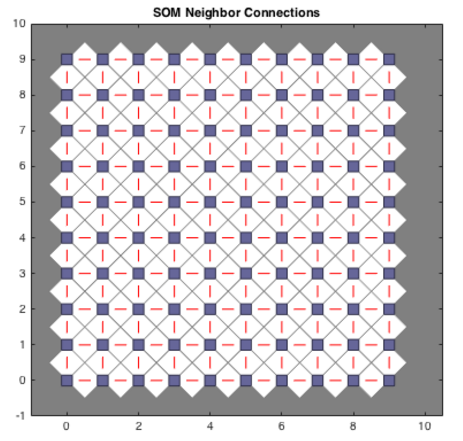
\includegraphics[width=.73\linewidth]{grid_top}
  \caption{Topologie organizovaná do pravoúhlé mřížky}
  \label{fig:sub2}
\end{subfigure}
\caption{Dvě možné topologie, modré značky představují neurony, zatímco červené spoje indikují sousedství}
\label{fig:top}
\end{figure}

\subsection{Učení}

Jak již bylo zmíněno, samoorganizující se mapa se učí bez učitele a to kompetitivním učením. Základní myšlenka učícího algoritmu je následující: síti se opakovaně předkládají vstupy a váhové vektory neuronů jsou upravovány tak, aby více odpovídaly rozložení původního prostoru.
% je jich více, jeden z algoritmů
Konkrétně lze učení popsat pseudokódem:

\begin{enumerate}
\item Inicializace vektorů.
\item Jeden vstupní vektor je předložen síti.
\item Je nalezen neuron, který má se vstupem nejpodobnější váhový vektor. Pro tuto podobnost se dá použít např. euklidovská vzdálenost. Takový neuron se nazývá Best matching unit (BMU).
\item Váhový vektor každého neuronu je pak přiblížen vstupnímu vektoru. Velikost tohoto příblížení je určena vztahem ().
Závisí tedy na vzdálenosti neuronu od BMU, meřené v mřížce -- čím dále jsou neurony od sebe, tím je přiblížení slabší. Dále velikost těchto změn slábnou s každou iterací učení. Celý vztah pro úpravu váhového vektoru W neuronu i je určen vztahem \ref{eq:1}.


\item Znovu body 2 - 5 po N iterací.
\end{enumerate}

\begin{equation} \label{eq:1}
\sum_{i=0}^{\infty} a_i x^i
\end{equation}

\begin{equation} \label{eq:weights_adjust}
\mathcal{W}_i(t+1) = \mathcal{W}_i(t) + \alpha \sigma(win, i, t)(\mathcal{X}(t) - \mathcal{W}_i(t))
 \begin{equation} 
\subsection{Vlastnosti}
SOM, stejně jako mnoho dalších dataminingových metod, předpokládá, že příslušnost tříd je definovaná podobností atributů.

Dále je chování samoorganizujících map ovlivněno počtem neuronů -- bylo ukázáno, že samoroganizující mapy s relativně malým počtem neuronů (oproti velikosti datasetu) se chovají podobně jako metoda K-means\cite{needed}. Prototypové vektory pak  představují středy shluků v původním prostoru.

Naopak pro sítě s počtem neuronů srovnatelným s počtem vstupních dat, SOM učením vytváří diskrétní reprezentaci vstupního prostoru -- \textit{mapu}, ktera zachovává topologické vlastnosti prostoru, založené na sousednosti (co bylo blízko ve vstupním prostoru bude blízko i na mapě).
% neighboorhood function



\subsection{Využití}

Jelikož se vlastnosti samoorganizujících map různí podle počtu použitých neuronů, využití se liší taktéž podle tohoto parametru.

SOM s malým počtem neuronů je možné využít tam, kde je možné použít K-means. \dots výhody, nevýhody, rozdíly


Naopak samoorganizující mapy s velkým\footnote{Velký počet v tomto smyslu představuje řádově srovnatelný s počtem vstupních vektorů.} počtem neuronů se používají převážně jako nástroj pro redukci dimenzionality.  Toho lze využít v transformaci dat při procesu KDD (\ref{subsec:transformace}), podobně, jako ostatní metody s tímto účelem\cite{som_dim_red}. Kterýkoliv vektor ze vstupního prostoru je namapován na pozici v mřížce -- ta je určena pozicí neuronu, který se aktivuje pro příslušný vstupní vektor, jinými slovy je pro něj BMU.


Dále je možné zkoumat naučenou \textit{mapu}. Tato mapa je určena prototypovými vektory neuronů, které mohou sloužit jako vstupní prostor pro další shlukovou analýzu\cite{som_clustering}. Dále je mapa, díky své nízké dimenzionalitě, vhodná pro vizualizace a 
\textit{explorační analýzu}\footnote{Explorační analýza představuje metody pro průzkum dat a hledání hypotéz.}, což je také nejrozšířenější použití samoorganizujích map.



\subsubsection*{Vizualizace map}
Vizualizace je mocný nástroj pro extrakci znalostí a hypotéz z dat, převážně protože do procesu zahrnuje lidské vnímání, zkušenosti a kreativitu, které jsou při takové činnosti klíčové\cite{visual}. Bohužel tyto lidské schopnosti, stejně tak jako možnosti vizualizace, jsou značně omezené, pokud jsou data vysoce dimenzionální. Jak již bylo zmíněno, samoorganizující mapy poskytují dvou-demenzionální reprezentaci dat, kterou je možné snadno vizualizovat.



http://stackoverflow.com/questions/18233994/interpreting-a-self-organizing-map


\section{CRSOM}
Context-relevant self organizing map, Samoorganizující mapa se zahrnutým sémantickým kontextem (CRSOM) je umělá neuronová síť navržena Pitoyo Hartonem. Narozdíl od kasické SOM se CRSOM učí s učitelem, z čehož vyplývá, že k učení je nutné znát dvojice vstupní a výstupní vektor. Právě výstupní vektory určují tzv. \textit{kontext učení}, což mohou být například třídy vstupních vektorů.

\subsection{Struktura sítě}
CRSOM se skládá ze tří vrstev neuronů. Prostřední (skrytá) vrstva je organizovaná do 2D mřížky neuronů, tzn. stejně jako u klasické samoorganizující mapy.
 Oproti SOM má CRSOM ještě jednu vrstu navíc -- výstupní (\textit{kontextovou}).  Každý neuron výstupní vrstvy je propojen s každým neuronem ve skryté SOM vrstvě (viz obr. \ref{fig:crsom_structure}). 
 

\begin{figure}[htbp]
\begin{center}
	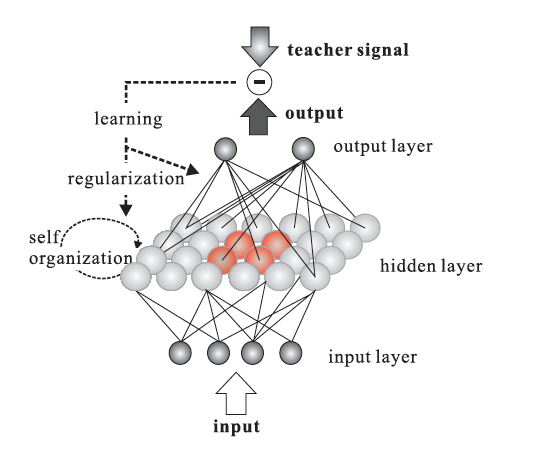
\includegraphics[scale=0.6]{crsom_structure}
\caption{}
\label{fig:crsom_structure}
\end{center}
\end{figure}
 
 

\subsubsection*{Výstup sítě}
Výstup celé sítě je složená funkce vstupního vektoru. 
Jínými slovy první z vrstev aplikuje svou funkci na vstupní vektor a každá další vrstva aplikuje svou funkci na výstup neuronů z předchozí vrstvy. Tento přístup je stejný jako u MLP.

V následujícím odstavci budou probrány jednotlivé funkce vrstev a jejich význam.

\subsubsection*{Výstup skryté vrstvy}
První funkce, jejíž vstupem je konkrétní vstupní vektor, je $ \mathcal{O}_h^i(t) $. Tato funkce představuje míru aktivace i-tého neuronu ve skryté vrstvě. $ \mathcal{O}_h^i(t) $ se skládá ze dvou multiplikativních členů.

$$ \mathcal{O}_h^i(t) = e^{-\mathcal{I}_i^h(t)} \sigma(win, i, t) $$

První z členů představuje vztah aktivace neuronu $i$  a podobnosti vstupního a příslušného váhového vektoru. Tato funkce zobrazuje vzdálenost dvou vektorů do intervalu $(0;1]$. Průběh této funkce je zobrazen na obr. (\ref{fig:exp}).

$$ \mathcal{I}_h^i(t) = \|\mathcal{X}(t)-\mathcal{W}_i(t)\|^2 $$

        \begin{description}
            \item[ $\mathcal{X}(t)$] vstupní vektor
            \item[ $\mathcal{W}_i(t)$] váhový vektor neuronu $i$
             \item[ $\|\|$] norma \dots
        \end{description}   


\begin{figure}[htbp]
\begin{center}
	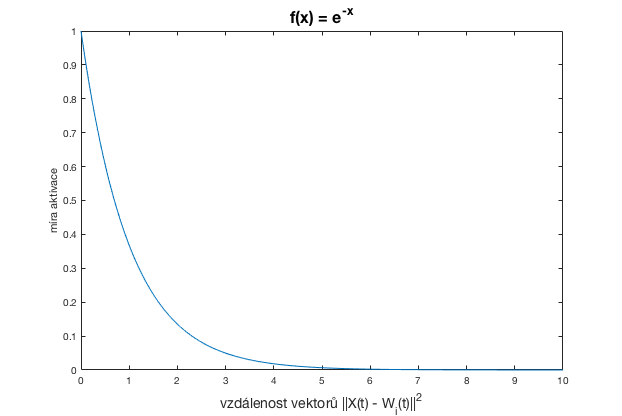
\includegraphics[scale=0.5]{exp.png}
\caption{Funkce, která zobrazuje vzdálenost vektorů do intervalu $(0;1]$}
\label{fig:exp}
\end{center}
\end{figure}
 

Druhý člen představuje topologickou restrikci v mapě neuronů. Jinými slovy jde o aktivování neuronů v závislosti na pozici v mřížce. Čím blíže je neuron k BMU, tím je tato aktivace vyšší, zároveň tato aktivace klesá s časem, které je zajištěné funkcí $s(t)$.  
V této praci byly parametry $s_0$ a $s_{end}$ nastaveny na $200$ a $0.01$, stejně tak, jak je navrženo a empiricky otestováno v originální publikaci \cite{hartono14}.

$$\sigma(win, i, t)=e^-\frac{dist(win, i)}{s(t)}$$
$$ {s(t)=s_0(\frac{s_{end}}{s_0})^\frac{t}{t_{end}}}$$ 

         \begin{description}
            \item[ $dist(win, i)$] vzdálenost BMU a neuronu $i$, měřeno na mřížce 
            \item[ $s_0, s_{end}$] $200$, $0.01$
             \item[ $t$] současná epocha
             \item[ $t_{end}$] počet epoch 
        \end{description}   

Na obrázku \ref{fig:top_restr} jsou zobrazeny tři mřížky neuronů. Každý z obrázků představuje výstup skryté vrstvy pro stejný vstup, ale v různých fázích učení (v různých epochách). Každá diskrétní pozice $(x, y)$ tedy představuje jeden neuron a velikost značky na pozici $(x, y)$ představuje relativní míru aktivace s tím, že BMU je v těchto případech na pozici  $(7, 7)$.

Grafy se liší pouze fází účení -- tedy epochou. V prvním případě je stav aktivace neuronů zobrazen na počátku učení, konkrétně v $8.$ epoše z celkových $50$. Graf dokumentuje skutečnost, že v této fázi jsou do formování mapy zahrnuty velkou měrou všechny neurony na mapě. V dalších dvou případech, které zobrazují stav ve $20.$ resp. $30.$ epoše, je rozpoznatelné zmenšující se okolí BMU, které je řízeno funkcí $s(t)$.




Oproti tomu na obr \ref{fig:sigma} je zobrazena závislost míry aktivace pro celý průběh učení pro fixní vzdálenost neuronů. V prvním grafu je vykreslena funkce $\sigma$ pro neurony vzdálené $1$, což se dá interpretovat jako míru topologické aktivace pro nejbližší neuron k BMU.
Na zbylých grafech jsou zobrazeny průběhy pro větší vzdálenost od BMU -- konkrétně $7$ a $25$. Z grafů je zřetelné, že vzdálené neurony od BMU se do formování mapy výrazněji zahrnují jen v počátečních fázích učení. Zahnutí neuronů pak strmě klesá a např. neurony vzdálené 25 se do formování mapy po 40. epoše zahrnují jen zanedbatelnou měrou.

\begin{figure}[htp]

\centering
\hspace*{-1cm}
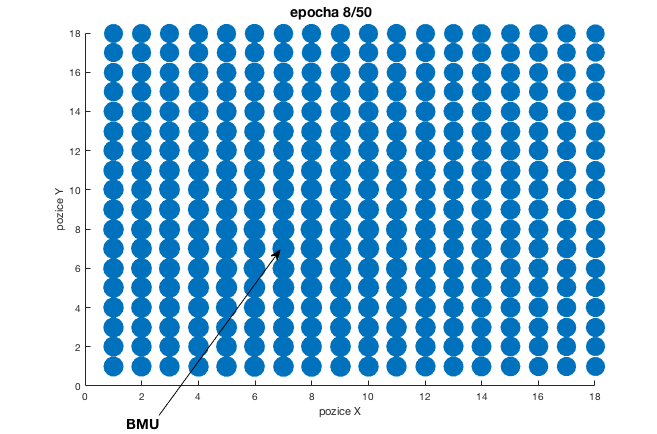
\includegraphics[width=.33\textwidth]{top_restr_8.png}\hspace*{-1cm}
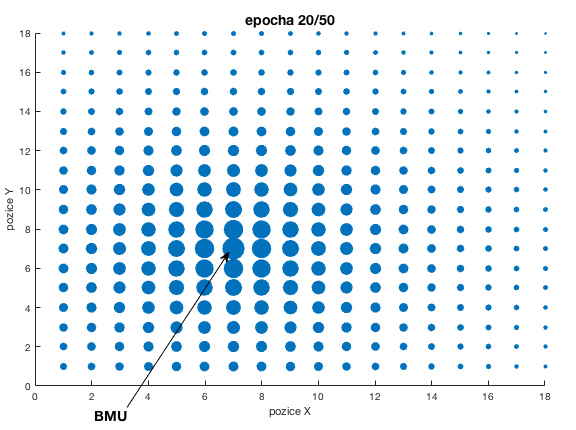
\includegraphics[width=.33\textwidth]{top_restr_20.png}\hspace*{-1cm}
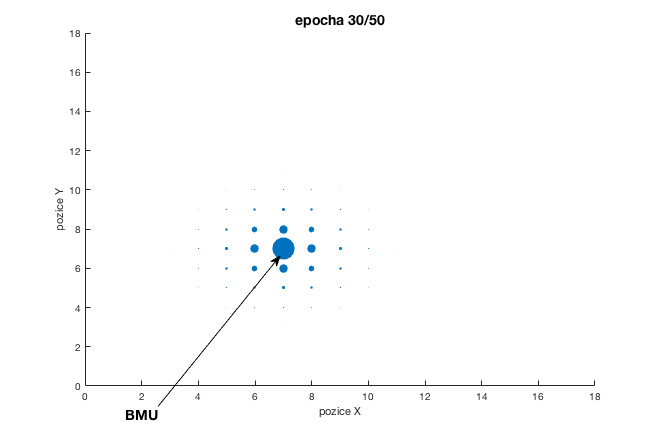
\includegraphics[width=.33\textwidth]{top_restr_30.png}
\hspace*{-1cm}
\caption{Příklad aktivace neuronů pro různé fáze učení.}
\label{fig:top_restr}

\end{figure}


\begin{figure}[htp]

\centering

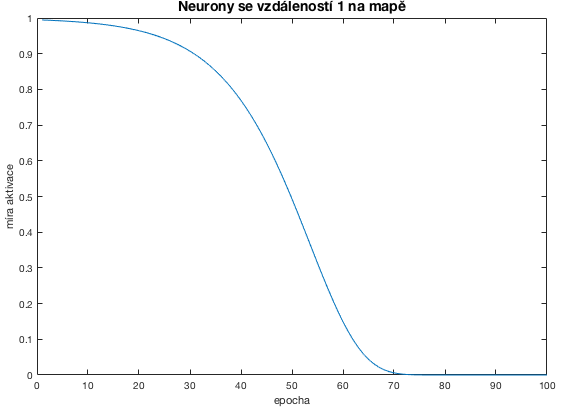
\includegraphics[width=.33\textwidth]{sigma_1.png}\hspace*{-1cm}
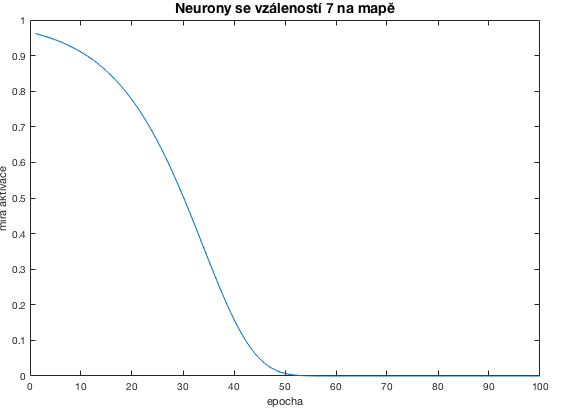
\includegraphics[width=.33\textwidth]{sigma_7.png}\hspace*{-1cm}
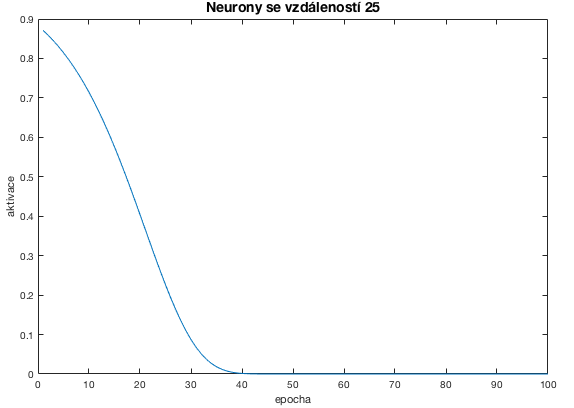
\includegraphics[width=.33\textwidth]{sigma_25.png}
\caption{Míra aktivace po celé učení pro různé vzdálenosti od BMU}
\label{fig:sigma}

\end{figure}


\subsubsection*{Výstupní vrstva}
Výstup neuronů skryté vrstvy slouží jako vstup do výstupní vrstvy sítě. Výstupní vrstva funguje jako jedna obyčejná vrstva MLP. Tedy výstup neuronu  $k$ ve výstupní vrstvě je dán funkcí $\mathcal{O}_k(t)$.

$$ \mathcal{O}_k(t) = f(\mathcal{I}_k(t))   $$
$$ \mathcal{I}_k(t) = \sum\limits_i{v_{ik}(t)\mathcal{O}_i^h - \theta_k(t)} $$


  
           \begin{description}
             \item[ $\theta_k(t)  $] bias pro neuron $k$
            \item[ $f(x) $] sigmoida 
        \end{description}  

 

\subsection{Učení}
Protože se CRSOM učí s učitelem, ke každému vstupnímu vektoru máme požadovaný výstupní vektor. Lze zavést funci $E(t)$, která bude sloužit jako chybová funkce.

 $$ E(t)=\frac{1}{2}\sum\limits_k{(\mathcal{O}_k(t)-\mathcal{T}_k(t))^2}$$

   \begin{description}
     \item[ $\mathcal{O}_k(t)$] výstup neuronu $k$
    \item[ $\mathcal{T}_k(t) $] požadovaný výstup pro neuron $k$
\end{description}  

Funkce $E(t)$ představuje chybu pro vstupní vektor a nastavení sítě v podobě vah. Jedním ze způsobů jak optimalizovat takovou funkci je \textit{metoda nejstrmějšího sestupu}, tedy pomocí gradientu funkce $E(t)$. Změny ve výstupní vrstvě -- tedy váhových vektorů $v_{ik}$ a biasu $ \theta_k$ -- se řídí podle následujících vztahů:


  $$ v_{ik}(t+1)=v_ik(t) - \eta_1\frac{\partial{E(t)}}{\partial{v_{ik}(t)}} =  v_{ik}(t) - \eta_1\delta_k(t)\mathcal{O}_h^i(t)  $$
  $$ \theta_k(t+1)=\theta_k(t) - \eta_1\frac{\partial{E(t)}}{\partial{\theta(t)}} = \theta(t)  + \eta_1\delta_k(t) $$
$$ \delta_k(t) = (O_k(t) - T_k(t))O_k(t)(1-O_k(t)) $$

     \begin{description}
        \item[ $\eta_1$] learning rate pro výstupní vrstvu
    \end{description}  
    

Stejným spůsobem se pak upravují i váhové vektory neuronů ve skryté vrstvě:
  
  $$ \mathcal{W}_i(t+1)=W_i(t) -  \eta_2\frac{\partial{E(t)}}{\partial{W_i(t)}} $$
	

	

$$\delta_i^h(t)=-e^{-I_i^h(t)}(\sum\limits_k{\delta_k(t)v_{ik}(t)}) $$
$$ \mathcal{W}_i(t+1)=\mathcal{W}_i(t) -  \eta_2\delta_i^h(t)\sigma(win, i, t)(\mathcal{X}(t) - \mathcal{W}_i(t)) $$


         \begin{description}
             \item[ $\eta_2$] learning rate pro skrytou vrstvu
            \item[ $\mathcal{X}(t)$] vstupní vektor
            \item[ $\mathcal{W}_i(t)$] váhový vektor neuronu $i$
        \end{description}  


 

\subsection{Srovnání se SOM }
\subsubsection*{Rozdíl ve formování SOM a CRSOM}
Narozdíl od vztahu, který popisuje úpravy prototypových vektorů v sítích typů SOM, se v úpravách prototypových vektorů CRSOM navíc vyskytuje člen $\delta_i^h(t)$.

Tento člen slouží jako \textit{regulační signál}, který je určen velikostí chyby na výstupu. Slouží tak jako zpětná vazba z kontextové sítě, která řídí formování skryté vrstvy podle zadaného kontextu.

Pouze v případě $ \delta_i^h(t) > 0 $, je neuron $i$ přiblížen ke vstupnímu vektoru. V případě $ \delta_i^h(t) < 0 $ je naopak oddálen. Z toho vyplývá, že ke vstupnímu vektoru jsou přiblíženy pouze prototypové vektory neuronů, které přispívají ke snížení chyby, ostatní jsou naopak pokutovány oddálením. V případě, že $ \delta_i^h(t) = 1 $, CRSOM simuluje chování SOM: prototypové vektory jsou ke vstupnímu vektoru přiblíženy vždy, bez ohledu na sémantický kontext a výstup sítě. Rozdílné formování sítě je doloženo na obr \ref{fig:dunno}.


\subsubsection*{Rozdíl v interpretaci SOM a CRSOM}
Samoorganizující mapy jsou schopné vysoce dimenzionální prostor mapovat do 2D a zachovat při tom některé topologické vlastnosti vstupního prostoru. Pokud máme k datům nějaký konktext (třídy) a chceme je nějakým způsobem využít pro formování mapy, není jiná možnost, než využít třídy jako další atributy. Naopak CRSOM s těmito informacemi zachází explicitně a pomocí těchto tříd prostřednictvím regulačního signálu řídí formování mapy podle zadaného kontextu. SOM je schopný vizualizovat prostor, zatímco CRSOM je schopná vizualizovat problém.\cite{hartono14}



\subsection{Vlastnosti a využití}

CRSOM naučená na konkrétní sémantický kontext může být využita jako klasifikátor tohoto kontextu pro nová data. V takovém případě mapa, která je definovaná skrytou SOM vrstou, představuje vedlejší produkt takového učení. Tato mapa nám dává intuitivní pochopení výkonnosti takového klasifikátoru.

Dále je možné považovat mapu jako cílový produkt učení a pokládat účel CRSOM jako definování mapování  N-dimenzionálního prostoru do dvou dimenzionálního, které bere v úvahu rozložení vstupního prostoru a využívá sémantický kontext. Vzniklá mapa pak může sloužit na vizualizování klasifikačního problému pro daný sémantický kontext. Dále je možné z mapy extrahovat znalosti a strukturu v podobě vytvořených shluků

% -------------------------------------- Návrh a implementace ---------------------------------------------------------------------------------------------------------------------------------------------------------------
\chapter{Návrh a implementace}

\section{SOM}


\subsection{Matlab}


\section{CRSOM}

Implementace CRSOM byla mnohem náročnější. Jedním z důvodů bylo to, že v době implementace bylo k dispozici pouze analytické vyjádření fungování sítě, bez jakékoliv vzorové implementace.
Správnost sítě tak bylo možné verifikovat pouze na základě výstupů z experimentů provedených Hartonem na známých datových sadách.\cite{hartono14}.

Další překážkou bylo, že prováděné experimenty byly spouštěny pro $30 000$ epoch, což by znamenalo několik dní výpočtů pro první naivní implementace.
	
Postup pro implementaci sítě tak, jak byla navržena Hartonem, byl inspirován přístupem \uv{Make it work, make it right, make it fast}.\cite{makeit} 
Tento přístup logicky prioritizuje vývoj software: jako první by měla být zaručena korektní implementace. Až poté je možné implementaci vylepšovat ve směrech designu, robustnosti a výkonu. Pro zachování správnosti software je nutné zavést regresní testování, které zaručí pokračující korektnost i po změnách v rámci \uv{Make it right} a \uv{make it fast}.

\subsection{Make it work}
 Jak bylo zmíněno, první naivní implementace sítě není možné verifikovat oproti Hartonovým experimentům, nadruhou stranu je z definice sítě a z dostupných publikací (např.: \cite{hartono14}) zřejmé, jak se bude mapa formovat pro jednoduché příklady. Takovým jednoduchým příkladem je například dobře známý dataset Iris. Tento dataset byl navíc omezen na $2$ dimenze, což nám poskytne možnost vizualizovat neurony, určené prototypovými vektory, spolu se vstupními daty v jednom grafu. Vizualizace formování se ukazala, jako velmi platná pro pochopení a ladění fungování sítě. Kromě zobrazování neuronů na mapě spolu se vstupními daty, byly ukládány a zanášeny do grafů další hodnoty významné pro průběh učení. Mezi takové hodnoty patří například hodnota funkce $E(t)$, průměrné výstupy neuronů ze skryté vrstvy, průměrná topologická restrikce a další.
 
Další překážkou byla vysoká citlivost metody na nastavení parametrů učení\cite{hartono14}. Slabé výsledky tak mohou být způsobeny nesprávným nastavením sítě a ne vždy musí znamenat chybu v implementaci. Tomuto problému bylo čeleno pomocí prohledávání prostoru parametrů a kontrolování všech výsledků, alespoň z počátku verifikace.
Pomocí těchto přístupů se podařilo naimplementovat CRSOM, která dávala srovnatelné výsledky na stejných datasetech podle originálních publikací \cite{hartono14}.

\subsection{Make it right and make it fast}

První verze sítě byla sice funkční, trpěla ale několika prohřešky jak z výkonového hlediska, tak z designového. Ještě před jakýmikoliv úpravami bylo nutné vytvořit sadu regresních testů, které budou zajišťovat stálou správnost sítě. Toho bylo docíleno odebráním všech nedeterministických nastavení a uložení stavu sítě po několika epochách učení \textit{(expected net)} pro daný testovací dataset.  Regresní testování upravené sítě pak spočívalo ve spuštění učení se stejným nastavením a pro stejný dataset jako pro síť \textit{expected net}. Za předpokladu deterministického učení, naučená síť musí mít stejné hodnoty prototypových vektorů jako \textit{expected net}.

Výkon sítě se měřil pomocí učení na datasetu, který byl výrazně větší, než dataset určený pro testování. K určení problémových míst implemetace, z hlediska výkonu, byl výhradně používán Matlab profiler, který je vestavěný do IDE. (pozn pod čarou: http://www.mathworks.com/help/matlab/matlab_prog/profiling-for-improving-performance.html). Zlepšování sítě bylo provádělo iteračně, postupné pokroky jsou zaneseny do tabulky (\dots). Od první naivní implementace se učení zrychlilo více než $15x$.  Nejvyšší pokroky ve výkonu byly dosaženy následujícími upravami:

\subsubsection*{Funkce adapt}

\subsubsection*{Maticové počítání}

\subsubsection*{Prealokace}


\subsection{Konečný design}


\section{Implementace experimentů}

Celý proces implementace a experimentování na cílových datech přineslo několik problémů, kterým bylo nutné čelit. 
Použitá data byla dostupná přes veřejné API a velikost jednoho surového záznamu byl poměrně veliký (stovky Kb).
Proces implementace si vynutil současnou existenci několika různých verzí sítě s rozdílným nastavení  parametrů. Z důvodu dlouhé prodlevy mezi změnou a výsledkem bylo nutné efektivně zaznamenávat důvod konkrétních změn a jejich kontext.
Samotné experimenty pak vyžadovaly časté spouštění trénování pro různé datové sady a různé nastavení parametrů učení. Výsledky experimentů pak bylo nutné jednoduše vyhodnocovat, třídit a ukládat. To vše ohledem na vysokou výpočetní a prostorovou náročnost metody a nemožností paralelizace na osobním stroji s jednou Matlab licencí. 


\subsection{Tvorba datasetů}

Je třeba zmínit, že všechny vytvořené datové sady pocházely z jednoho zdroje. Z důvodu poměrně objemných záznamů bylo vhodné tato data cachovat do lokální databáze. Pro tento účel byla zvolena MongoDb databáze. Samotné stahování dat z API a generování datasetů bylo docíleno skripty v programovacím jazyce Ruby. V této sekci budou představeny tyto klíčové technologie spolu s důvodněním jejich výběru. Spolupráci technologií při stahování dat z API následné generování datasetů je pak zobrazena na obr. \ref{fig:down}.

\begin{figure}[htbp]
\begin{center}
	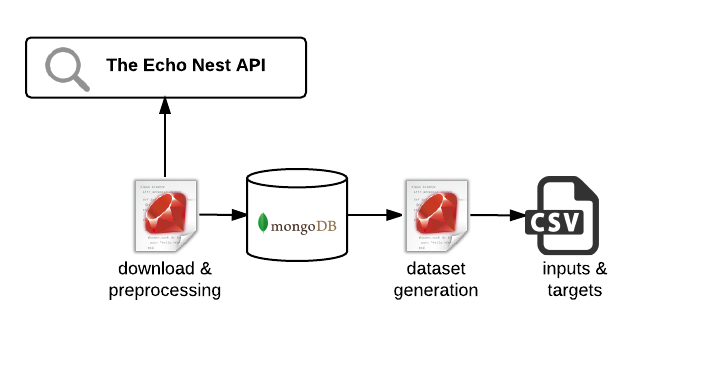
\includegraphics[scale=1]{download_generate.png}
\caption{Stahování dat z API a generování datasetů}
\label{fig:down}
\end{center}
\end{figure}

\subsubsection*{MongoDb}
MongoDb je dokumentově orientovaná databáze, tedy patří mezi tzv. NoSql databáze. MongoDB umožňuje ukládat data bez dopředu známého schématu, což byl nejvýznamější důvod pro použití právě takové databáze v rámci této práce.

Data v MongoDb jsou interně uložena a navenek prezentována ve formátu BSON, což je specifikace a knihovna pro převod JSONu do binární podoby. Data, která poskytuje The Echo Nest prostřednictvím webového API, jsou taktéž ve formátu JSON, Tato skutečnost dělá dokumentovou databázi mnohem lepším kandidátem, než by tomu byly tradiční relační databáze. Navíc, pro využítí databáze jako lokální cache, jsou nepotřebné další vlastnosti, které nabízejí relační databáze, jako jsou transakční zpracování, integritní omezení a další.

\subsubsection*{Ruby}
Pro ukládání dat do MongoDB a následné generování datasetů ve formátu csv by zvolen jazyk Ruby. Ruby je interpretovaný skriptovací jazyk, který vznikl v roce 1995 v Japonsku.
Jazyk Ruby byl zvolen pro svou jednoduchou syntax, možnost krátkého zápisu kódu a širokou dostupnost gemů (pozn: \dots). Jedním takovým gemem, který byl použit je Mongoid, který slouží jako ODM (Object-Document-Mapper) framework pro databázi MongoDb.
Jednou ze slabých stránek jazyka Ruby je výkon \cite{ruby_performance}, alespoň ve srovnání s kompilovanými jazyky jako je např C++. Tato nevýhoda je ovšem pro toto konkrétní použítí nevýznamná, naopak snadný zápis kódu a dostupnost gemů znamená obrovskou časovou úsporu a snadnou modifikaci kódu.


\subsection{Framework na experimenty}
Jak již bylo zmíněno, velké množství experimetů pro různé verze kódu a konfigurace metod přinesly spousty požadavků. Mezi požadavky mimo jiné patřilo napřiklad jednoduché nasazování kódu, logování  …\dots…. . Pro naplnění těchto požadavků byly zvoleny dvě hlavní technologie: výpočetní centrum MetaCentrum a verzovací nástroj Git.


\subsubsection*{MetaCentrum}
Metacentrum je projekt Cesnetu, který v České republice zastřešuje většinu aktivit, souvisejících se superpočítáním. Má k disposici řadu výpočetních clusterů, které může mít k disposici prakticky každý člověk z akademického prostředí.
Na strojích MetaCentra běží Unixové operační systémy, které je možné ovládat vzdáleně z příkazového řádku. MetaCenrum obsahuje dva druhy uzlů: jedním druhem jsou tzv. \textit{čelní uzly}.
Na čelní uzly je možné se přihlásit a zadávat úlohy spolu s požadavky na zdroje v podobě úložiště, paměti, CPU a další.
Druhým typem jsou \textit{výpočetní uzly}, které jsou vytěžovány plánovacím systémem \textit{Torque}. Torque dohlíží na efektivní a férové využívání zdrojů uživateli, a plánuje, kdy kdo dostane vyžádané stroje k dispozici. \cite{metacentrum}

\subsubsection*{Git}
Git je distribuovaný systém správy verzí. Git umožňuje snadným způsobem uchovávat různé verze souboru spolu s jejich kompletní historií. Nová verze se vytváří tzv. \textit{větvemi (branch)}, ucelené změny v souborech se nazývají \textit{commity}, které také obsahují krátký text, který změnu kometuje. 


\subsubsection*{Zadávání úloh}
Z důvodu vysoké náročnosti úloh na prostředky byly v drtivé většině případů všechny sítě učeny na výpočetních uzlech v MetaCentru. Pro spuštění učení sítí pro jeden dataset je nutné mít v MetaCentru k dispozici kód v matlabu, vstupní soubory a skript, který zadá úlohy s různými parametry učení. Všechna tato data byla do MetaCentra dopravena přes vzdálený Git repozitář. Jeden experiment tak spočíval ve vytvoření commitu, který byl dopraven přes vzdálený repozitář do MetaCentra. V MetaCentru pak byl spuštěn skript, který zadal úlohy. Všechna tato práce lze automatizovat jedním bash skriptem (\ref{fig:up}). 
Jednou z výhod takového přístupu je uchování kompletní historie experimentů spolu se smysluplnými komentáři, které lze generovat strojově. Přiklad takového vygenerovaného komentáře (obr. \ref{fig:semantic_commit}) je část skriptu, který zadává úlohy s různými parametry učení. Dále jsou automaticky generována jména sítí -- jako složenina datasetu a parametrů učení. Toto jméno je pak použito jako identifikátor úlohy pro snadnou inspekci dostupnou přes uživatelské rozhraní MetaCentra. Dále je jméno použito na pojmenovávání vytvářených souborů -- např. logu, kdo kterého se ukládají informace o současné epoše a chybě.

\begin{figure}[htbp]
\begin{center}
	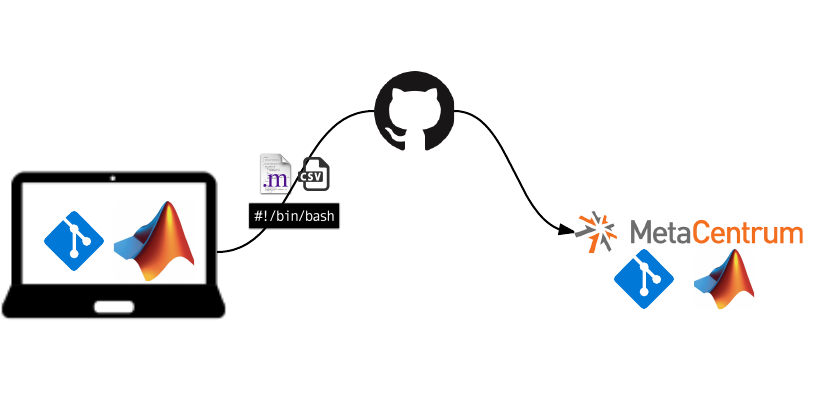
\includegraphics[scale=0.9]{up.png}
\caption{Zadávání úloh do MetaCentra}
\label{fig:up}
\end{center}
\end{figure}


\begin{figure}[htbp]
\begin{center}
	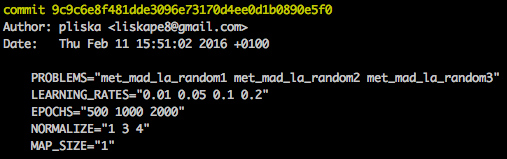
\includegraphics[scale=0.7]{semantic_commit}
\caption{Příklad strojově generovaného komentáře}
\label{fig:semantic_commit}
\end{center}
\end{figure}



\subsubsection*{Vyzvedávání výsledků}
Kromě logů jsou do souborového systému v MetaCentru ukládany také další soubory. Po dokončení učení je celý \textit{workspace} serializován a uložen na disk. Stejně tak je uložena vizualizace výsledků. Protože jsou tyto výsledky uloženy na disku, je snadné je prostřednictvím Gitu přenést zpět na lokální stroj (\ref{fig:down}). Zpravidla jsou nejdříve přenášeny výsledky v obrázkových podobách -- slouží jako rychlé náhledy na výsledky. Po zhodnocení výsledků je možné vybrat konkrétní uložené workspace a přenést na lokální stroj pro další inspekci a vizualizace.

\begin{figure}[htbp]
\begin{center}
	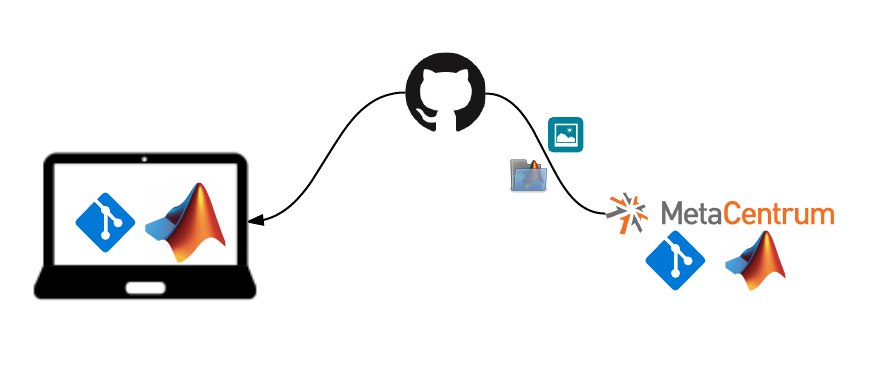
\includegraphics[scale=0.9]{down.png}
\caption{Příklad strojově generovaného komentáře}
\label{fig:down}
\end{center}
\end{figure}


% -------------------------------------- POUŽITÁ DATA ---------------------------------------------------------------------------------------------------------------------------------------------------------------
\chapter{Použitá data}
\section{Úvod do hudební problematiky}
Timbre and  pitch

% https://www.youtube.com/watch?v=mE1ZwLTZ1Bw


\section{MillionSongDataset a The Echo Nest}
MillionSongDataset je volně dostupná kolekce hudebních atributů a metadat pro více než milion skladeb populární hudby. Tento dataset je vytvořený za účelem podpory výzkumu v oblastech algoritmů pro hudební data, MRI a další. MillionSongDataset byl vytvořen společností The Echo Nest, která se zabývá hudební analýzou, porozuměním hudebního obsahu a vztahem hudby a posluchači. MillionSongDataset slouží jako zkratka k hudebním datům, které jinak The Echo Nest poskytuje prostřednictvím svého webového API.

	Při náročnosti používaných metod v této práci, je zřejmé, že není možné použít celý tento dataset, který má přibližně 280GB. S takto velkým objemem dat je také velmi komplikovaná manipulace. Nejen z těchto důvodů byl využit konkrétní zdroj dat a to již zmíněné API. Tímto přístupem je možné jednoduše vytvářet datasety pro předem zvolené sémantiky. Takové sémantiky mohou být například žánr hudby, období vzniku, oblíbenost, autor a další. Další výhodu, kterou přinesl tento přístup, je vyšší aktuálnost metadat, zejména těch, které jsou odvozeny na základě aktuálních trendů a sociálního vnímání jako je například oblíbenost konkrétní skladby nebo míra známosti hudebního autora.
	
\section{Dostupné atributy}
\subsection{Nástroj Analyze}

Analyze je nástroj pro analýzu hudebních dat, který používá společnost The Echo Nest. 
Tento nástroj je volně dostupný prostřednictvím webového API. Vstupem programu je digitální audio soubor (např.:  mp3, m4a, wav, mpeg, flv), který je programem analyzován. Výstupní informace programu jsou poskytuty JSON souborem, který popisuje strukturu nahrávky a hudební obsah včetně rytmu, výšek a tónů. Program využívá techniniky pro simulování fyzického a kognitivního vnímání hudby člověkem. Konkrétní fungování programu je ale proprietární. 

Příklad schématu JSON souboru, který popisuje skladbu Billie Jean je :TODO:. Pro účely této práce je nejdůležitější analýza s názvem “segments”. Jeden segment představuje množinu zvukových entit, které jsou relativně neměnné v hudebních atributech. Segmenty jsou charakterizovány začátkem a trváním v sekundách, hlasitostí a popisem výšek a tónů.

\begin{description}
\item[loudness] 
\item[pitches] 
\item[timbre] Nástroj Analyze popisuje timbre jako 12-dimezionální vektor. Pro účely této práce je důležité, že takové vektory jsou vhodné na porovnávání mezi sebou. Toto tvrzení a další informace o způsobu získávání vektorů, které je mimo rámec této práce, jsou k naleznutí v oficiální dokumentaci nástroje \cite{analyze}.
\item[confidence] desetinné číslo mezi 0 a 1, které symbolizuje jistotu analyzátoru pro konkrétní atribut. Z důvodu zjednodušení nebude v této práci tento atribut vůbec uvažován.
\end{description}

\subsection{Další atributy}
Mimo akustické atributy, které je možné získat z nástroje Analyze, The Echo Nest poskytuje velké množství dalších prostřednictví svého webového API.

Poskytované atributy je možné rozdělit do tří kategorií. První kategorie jsou metadata. Do této kategorie patří například název skladby, jméno autora nebo rok vzniku. Další kategorií jsou atributy tzv.: socilání. Do sociálních atributů jsou zařazeny míry oblíbenosti, známosti apod. Poslední kategorií jsou algoritmicky získané atributy, které popisují sladbu jako celek. Příkladem takových atributů jsou danceability (míra vhodnosti skladby pro tancování) a valence (míra pozitivní energie, kterou skladba vyzařuje). Vyčerpávající popis dostupných atributů je k nalezení: ()


% -------------------------------------- Experimenty ---------------------------------------------------------------------------------------------------------------------------------------------------------------
\chapter{Experimenty}


% -------------------------------------- Využití ---------------------------------------------------------------------------------------------------------------------------------------------------------------
\chapter{Využití}

\begin{conclusion}
	%sem napište závěr Vaší práce
\end{conclusion}

\bibliographystyle{csn690}
\bibliography{mybibliographyfile}

\appendix

\chapter{Seznam použitých zkratek}
% \printglossaries
\begin{description}
	\item[GUI] Graphical user interface
	\item[XML] Extensible markup language
\end{description}


% % % % % % % % % % % % % % % % % % % % % % % % % % % % 
% % Tuto kapitolu z výsledné práce ODSTRAŇTE.
% % % % % % % % % % % % % % % % % % % % % % % % % % % % 
% 
% \chapter{Návod k~použití této šablony}
% 
% Tento dokument slouží jako základ pro napsání závěrečné práce na Fakultě informačních technologií ČVUT v~Praze.
% 
% \section{Výběr základu}
% 
% Vyberte si šablonu podle druhu práce (bakalářská, diplomová), jazyka (čeština, angličtina) a kódování (ASCII, \mbox{UTF-8}, \mbox{ISO-8859-2} neboli latin2 a nebo \mbox{Windows-1250}). 
% 
% V~české variantě naleznete šablony v~souborech pojmenovaných ve formátu práce\_kódování.tex. Typ může být:
% \begin{description}
% 	\item[BP] bakalářská práce,
% 	\item[DP] diplomová (magisterská) práce.
% \end{description}
% Kódování, ve kterém chcete psát, může být:
% \begin{description}
% 	\item[UTF-8] kódování Unicode,
% 	\item[ISO-8859-2] latin2,
% 	\item[Windows-1250] znaková sada 1250 Windows.
% \end{description}
% V~případě nejistoty ohledně kódování doporučujeme následující postup:
% \begin{enumerate}
% 	\item Otevřete šablony pro kódování UTF-8 v~editoru prostého textu, který chcete pro psaní práce použít -- pokud můžete texty s~diakritikou normálně přečíst, použijte tuto šablonu.
% 	\item V~opačném případě postupujte dále podle toho, jaký operační systém používáte:
% 	\begin{itemize}
% 		\item v~případě Windows použijte šablonu pro kódování \mbox{Windows-1250},
% 		\item jinak zkuste použít šablonu pro kódování \mbox{ISO-8859-2}.
% 	\end{itemize}
% \end{enumerate}
% 
% 
% V~anglické variantě jsou šablony pojmenované podle typu práce, možnosti jsou:
% \begin{description}
% 	\item[bachelors] bakalářská práce,
% 	\item[masters] diplomová (magisterská) práce.
% \end{description}
% 
% \section{Použití šablony}
% 
% Šablona je určena pro zpracování systémem \LaTeXe{}. Text je možné psát v~textovém editoru jako prostý text, lze však také využít specializovaný editor pro \LaTeX{}, např. Kile.
% 
% Pro získání tisknutelného výstupu z~takto vytvořeného souboru použijte příkaz \verb|pdflatex|, kterému předáte cestu k~souboru jako parametr. Vhodný editor pro \LaTeX{} toto udělá za Vás. \verb|pdfcslatex| ani \verb|cslatex| \emph{nebudou} s~těmito šablonami fungovat.
% 
% Více informací o~použití systému \LaTeX{} najdete např. v~\cite{wikilatex}.
% 
% \subsection{Typografie}
% 
% Při psaní dodržujte typografické konvence zvoleného jazyka. České \uv{uvozovky} zapisujte použitím příkazu \verb|\uv|, kterému v~parametru předáte text, jenž má být v~uvozovkách. Anglické otevírací uvozovky se v~\LaTeX{}u zadávají jako dva zpětné apostrofy, uzavírací uvozovky jako dva apostrofy. Často chybně uváděný symbol "{} (palce) nemá s~uvozovkami nic společného.
% 
% Dále je třeba zabránit zalomení řádky mezi některými slovy, v~češtině např. za jednopísmennými předložkami a spojkami (vyjma \uv{a}). To docílíte vložením pružné nezalomitelné mezery -- znakem \texttt{\textasciitilde}. V~tomto případě to není třeba dělat ručně, lze použít program \verb|vlna|.
% 
% Více o~typografii viz \cite{kobltypo}.
% 
% \subsection{Obrázky}
% 
% Pro umožnění vkládání obrázků je vhodné použít balíček \verb|graphicx|, samotné vložení se provede příkazem \verb|\includegraphics|. Takto je možné vkládat obrázky ve formátu PDF, PNG a JPEG jestliže používáte pdf\LaTeX{} nebo ve formátu EPS jestliže používáte \LaTeX{}. Doporučujeme preferovat vektorové obrázky před rastrovými (vyjma fotografií).
% 
% \subsubsection{Získání vhodného formátu}
% 
% Pro získání vektorových formátů PDF nebo EPS z~jiných lze použít některý z~vektorových grafických editorů. Pro převod rastrového obrázku na vektorový lze použít rasterizaci, kterou mnohé editory zvládají (např. Inkscape). Pro konverze lze použít též nástroje pro dávkové zpracování běžně dodávané s~\LaTeX{}em, např. \verb|epstopdf|.
% 
% \subsubsection{Plovoucí prostředí}
% 
% Příkazem \verb|\includegraphics| lze obrázky vkládat přímo, doporučujeme však použít plovoucí prostředí, konkrétně \verb|figure|. Například obrázek \ref{fig:float} byl vložen tímto způsobem. Vůbec přitom nevadí, když je obrázek umístěn jinde, než bylo původně zamýšleno -- je tomu tak hlavně kvůli dodržení typografických konvencí. Namísto vynucování konkrétní pozice obrázku doporučujeme používat odkazování z~textu (dvojice příkazů \verb|\label| a \verb|\ref|).
% 
% \begin{figure}\centering
% 	
\includegraphics[width=0.5\textwidth, angle=30]{cvut-logo-bw}
% 	\caption[Příklad obrázku]{Ukázkový obrázek v~plovoucím prostředí}\label{fig:float}
% \end{figure}
% 
% \subsubsection{Verze obrázků}
% 
% % Gnuplot BW i barevně
% Může se hodit mít více verzí stejného obrázku, např. pro barevný či černobílý tisk a nebo pro prezentaci. S~pomocí některých nástrojů na generování grafiky je to snadné.
% 
% Máte-li například graf vytvořený v programu Gnuplot, můžete jeho černobílou variantu (viz obr. \ref{fig:gnuplot-bw}) vytvořit parametrem \verb|monochrome dashed| příkazu \verb|set term|. Barevnou variantu (viz obr. \ref{fig:gnuplot-col}) vhodnou na prezentace lze vytvořit parametrem \verb|colour solid|.
% 
% \begin{figure}\centering
% 	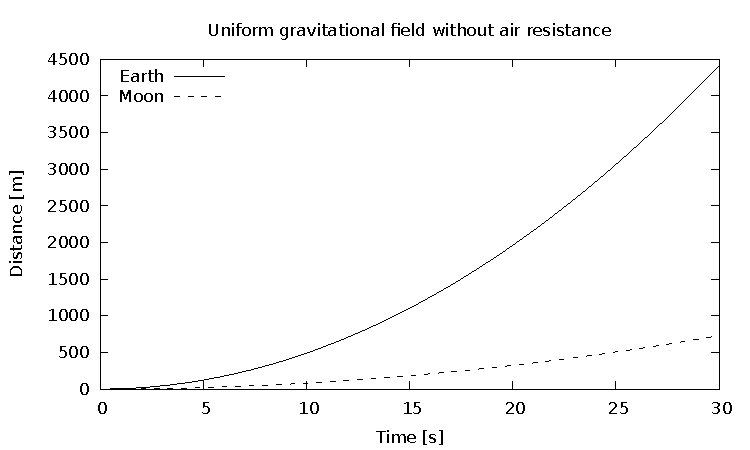
\includegraphics{gnuplot-bw}
% 	\caption{Černobílá varianta obrázku generovaného programem Gnuplot}\label{fig:gnuplot-bw}
% \end{figure}
% 
% \begin{figure}\centering
% 	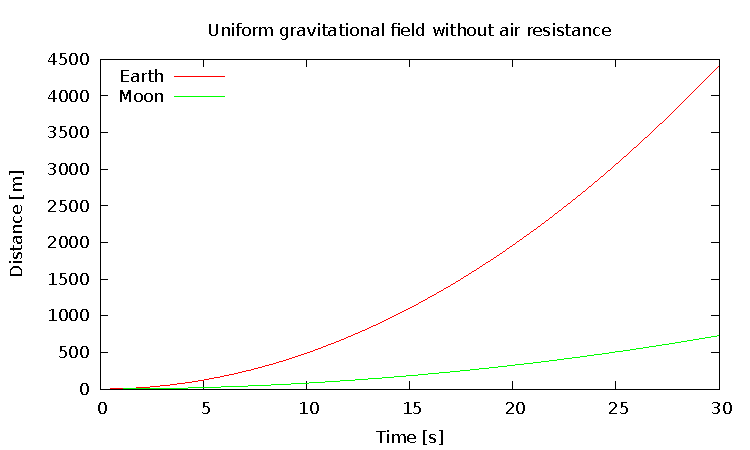
\includegraphics{gnuplot-col}
% 	\caption{Barevná varianta obrázku generovaného programem Gnuplot}\label{fig:gnuplot-col}
% \end{figure}
% 
% 
% \subsection{Tabulky}
% 
% Tabulky lze zadávat různě, např. v~prostředí \verb|tabular|, avšak pro jejich vkládání platí to samé, co pro obrázky -- použijte plovoucí prostředí, v~tomto případě \verb|table|. Například tabulka \ref{tab:matematika} byla vložena tímto způsobem.
% 
% \begin{table}\centering
% 	\caption[Příklad tabulky]{Zadávání matematiky}\label{tab:matematika}
% 	\begin{tabular}{|l|l|c|c|}\hline
% 		Typ		& Prostředí		& \LaTeX{}ovská zkratka	& \TeX{}ovská zkratka	\tabularnewline \hline \hline
% 		Text		& \verb|math|		& \verb|\(...\)|	& \verb|$...$|		\tabularnewline \hline
% 		Displayed	& \verb|displaymath|	& \verb|\[...\]|	& \verb|$$...$$|	\tabularnewline \hline
% 	\end{tabular}
% \end{table}
% 
% % % % % % % % % % % % % % % % % % % % % % % % % % % % 

\chapter{Obsah přiloženého CD}

%upravte podle skutecnosti

\begin{figure}
	\dirtree{%
		.1 readme.txt\DTcomment{stručný popis obsahu CD}.
		.1 exe\DTcomment{adresář se spustitelnou formou implementace}.
		.1 src.
		.2 impl\DTcomment{zdrojové kódy implementace}.
		.2 thesis\DTcomment{zdrojová forma práce ve formátu \LaTeX{}}.
		.1 text\DTcomment{text práce}.
		.2 thesis.pdf\DTcomment{text práce ve formátu PDF}.
		.2 thesis.ps\DTcomment{text práce ve formátu PS}.
	}
\end{figure}

\end{document}
